\documentclass[11pt,a4paper]{article}

\usepackage{geometry} \geometry{left=2.2cm, right=2.2cm, top=2.2cm, bottom=2cm}
\parskip 0.15cm 
\setlength{\parindent}{0cm} 
\usepackage{pdflscape}
\usepackage[document]{ragged2e}

\usepackage[T1]{fontenc}  % Set font

\usepackage{lineno}  % Line numbers

\usepackage{amssymb}  % Symbols
\usepackage{amsmath}
\usepackage{siunitx}

\linespread{1.25}  % Linespacing

\usepackage{xcolor} \newcommand{\todo}[1]{\textcolor{red}{\textbf{#1}}}   %

% Tables
\usepackage{multirow} \setlength{\tabcolsep}{4pt}

% Image handling
\usepackage{graphicx} 

\makeatletter \g@addto@macro\@floatboxreset\centering  
\makeatother

\graphicspath{ {img/} }  % Define image path

\usepackage{subfig}  % Compound figures

\usepackage{float}  % Precise figure location

% Bibliography management
\usepackage[style=authoryear, natbib=true, backend=biber]{biblatex}
\addbibresource{workflow.bib}

% Links within document, nice figure formatting
\usepackage[breaklinks]{hyperref} \definecolor{links}{RGB}{0,0,0} \hypersetup{
	breaklinks, colorlinks=true, linkcolor=links, anchorcolor=links,
	citecolor=links, filecolor=links, menucolor=links, runcolor=links,
	urlcolor=links, pdfauthor={John L. Godlee} }
	\def\subsectionautorefname{section} \def\subsubsectionautorefname{section}

% Variables
\title{Estimation of woodland canopy structure with terrestrial LiDAR: expanded methods}
\author{John L. Godlee}
\date{}

% Body
\begin{document}

\maketitle{}

\tableofcontents{}

\section{Introduction}

This document provides detailed field and analytical methods for the study of tree canopy structure in southern African woodlands. The study aimed to understand the effects of tree species diversity and composition on tree canopy structure and grassy biomass. Chapter XXX contains these methods in brief.

\section{Sampling}

Fieldwork was conducted at two sites, the first in Bicuar National Park, southwest Angola (S15.1$^\circ$, E14.8$^\circ$), and the second in and around Mtarure Forest Reserve, southeast Tanzania (S9.0$^\circ$, E39.0$^\circ$). Fieldwork was conducted during the peak growth period of each site, in order to capture the highest foliage volume in the canopy and the largest grass volume in the understorey.

\begin{figure}[H]
\centering
	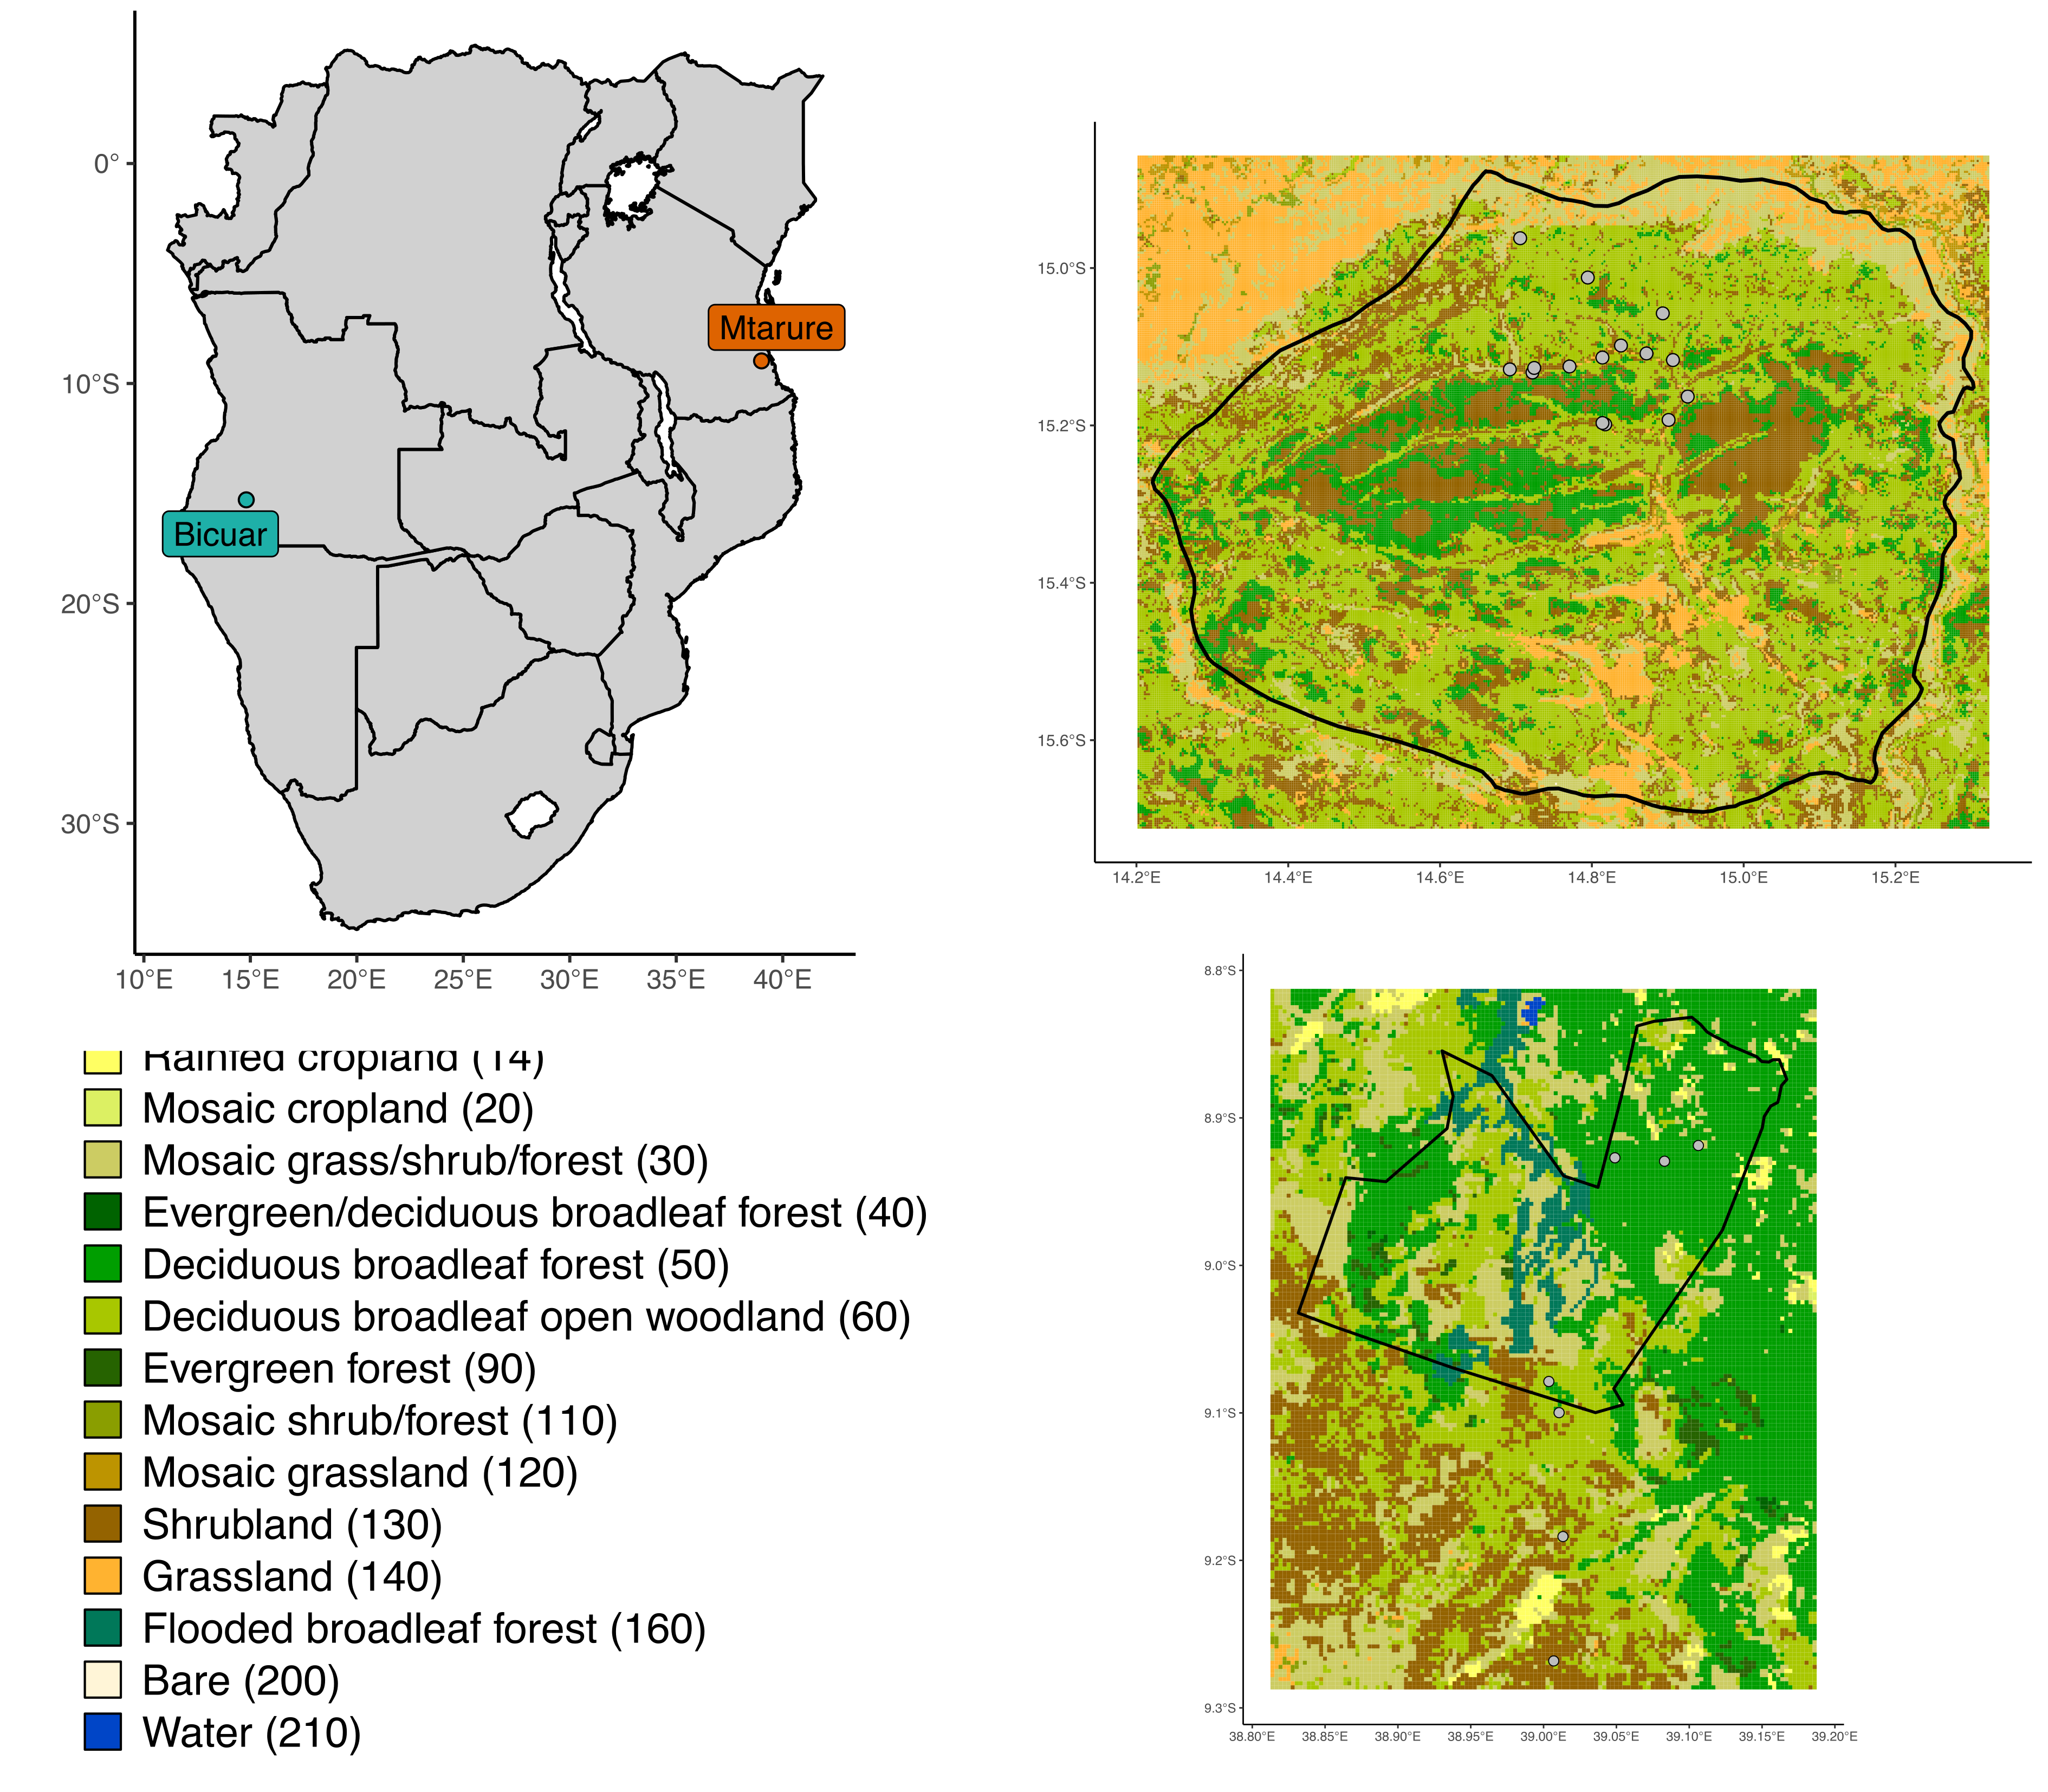
\includegraphics[width=\textwidth]{map}
	\caption{Location of study sites within southern Africa (a), and of 1 ha plots within each site. The blue polygons denote the boundaries of protected areas which encompass the majority of study sites, Bicuar National Park in Angola (b), and Mtarure Forest Reserve in Tanzania (c).}
	\label{map}
\end{figure}

% latex table generated in R 4.0.2 by xtable 1.8-4 package
% Mon Apr 19 15:05:58 2021
\begin{table}
\centering
\begin{tabular}{rcccc}
  \hline
site & mat & map & temp_range & cwd \\ 
  \hline
Bicuar & 20.8 (0.70) & 825.9 (52.01) & 24.5 (0.90) & -844.8 (44.29) \\ 
  Mtarure & 25.7 (0.24) & 958.4 (25.19) & 12.0 (0.33) & -739.6 (8.06) \\ 
   \hline
\end{tabular}
\caption{Climatic data for each site, extracted from WorldClim at 2.5 minute resolution. Values are the mean and standard deviation (in brackets) of all pixels intersecting each protected area.} 
\label{clim}
\end{table}



At each site, 1 ha permanent plots were sampled. In Angola, 15 plots were sampled, while in Tanzania, only seven were sampled, following the curtailment of fieldwork due to COVID-19 travel restrictions. Permanent plots were located in areas of homogeneous vegetation type, away from roads and undisturbed by humans, following the SEOSAW protocol (version 3.0). Plots were located quasi-randomly by first locating areas from satellite imagery expected to comprise savanna woodland vegetation. At each site, plots were deliberately located along a gradient of stem density.

Each permanent plot was further subdivided into nine 10 m diameter circular subplots arranged in a regular grid, with a buffer from the plot edge (\autoref{subplot}).

\begin{figure}[H]
\centering
	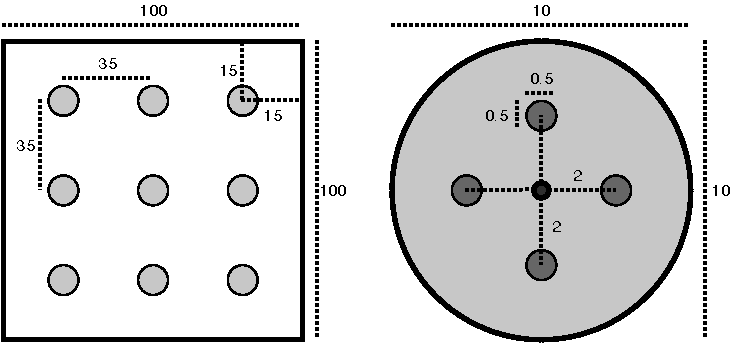
\includegraphics[width=\textwidth]{subplot}
	\caption{The layout of 10 m diameter subplots within each 1 ha square plot. Each subplot is situated inside a 15 m buffer from the plot edge, with 35 m between subplot centres. Subplots are arranged in a 3x3 grid. Disc-pasture measurements and biomass samples are located in cardinal directions 2 m from the centre of the subplot. All distances are in metres.}
	\label{subplot}
\end{figure}

\section{Field measurements}

\subsection{Trees}

For each subplot, we measured all woody stems >5 cm trunk diameter with canopy material inside the subplot. For each stem we measured:

\begin{itemize}
	\item{Tree identity}
	\item{Trunk diameter (Diameter at breast height - 1.3 m)}
\end{itemize}

For each tree, which may be composed of multiple stems, we measured: 

\begin{itemize}
	\item{Species}
	\item{Height to top of canopy}
	\item{Canopy area, ellipse from two perpendicular measurements (\autoref{crown})}
	\item{Distance from subplot centre}
	\item{Compass direction from subplot centre}
\end{itemize}

\begin{figure}[H]
\centering
	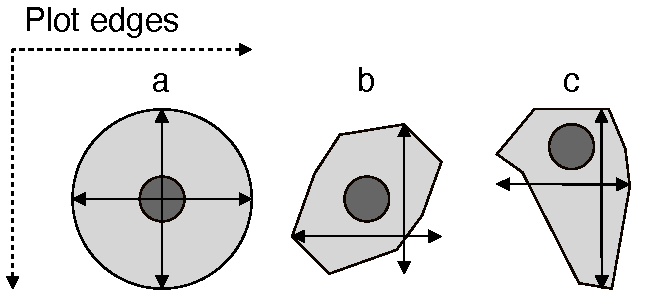
\includegraphics[width=\textwidth]{crown}
	\caption{Examples of tree crowns as viewed from above to demonstrate how crown extent measurements are located. Darker grey circles show the main trunk. Extent measurements are taken parallel to the plot edge. a) shows a perfectly circular tree crown, b) and c) show irregular tree crowns, demonstrating that maximum crown extent in a given orientation be offset from the trunk.}
	\label{crown}
\end{figure}

\subsection{Grass} 

Grassy volume and biomass within each subplot was estimated from four sample points located 2 m from the subplot centre in cardinal directions (\autoref{subplot}). At each point, a disc-pasture meter measurement was taken with a 45.8 cm radius disc weighing exactly 1.5 kg \citep{Bransby1977}. Small woody stems were removed from disc-pasture sample points before the disc-pasture measurement was taken. The location of the sample point was moved if the designated point intersected with coarse woody debris, rocks, immovable shrubs, or standing trees. Within each 1 ha plot, biomass harvesting was conducted at nine randomly allocated disc-pasture sample points. Tree leaf litter was removed from biomass samples. Grass samples in Angola were dried until the mass remained constant ($\pm$5 g) for >48 hours, then weighed to ascertain the grassy biomass. Grass samples from Tanzania could not be processed due to curtailment of fieldwork due to COVID-19 travel restrictions. 

\subsection{Hemispherical photography}

At the centre of each subplot a single photograph was taken with a Nikon D750 full-frame DSLR camera, with a circular fisheye lens. The lens had an equisolid (equal area) projection, which avoids image distortion. The projection function is given by: 

\begin{equation}
	R = 2f \sin{(\theta{}/2)}
\end{equation}

Where $R$ is the radial position of a point on the image on the sensor, $f$ is the focal length of the lens, and $\theta{}$ is the angle in radians of the desired angular radius of the cropped image. 

The photo was taken facing directly to zenith, with the top of the camera facing to magnetic north, at a height of 1.3 m or above understorey vegetation, whichever was higher. \autoref{camera_settings} shows describes the camera settings for each hemispherical photo:

\begin{table}[H] \centering 
  \caption{Description of camera settings used for each hemispherical photo. Note that the values of shutter speed and ISO are deliberately variable within sensible thresholds to adapt to light conditions.} 
  \label{camera_settings} 
\begin{tabular}{@{\extracolsep{0pt}} rl} 
\\[-1.8ex]\hline 
\hline \\[-1.8ex] 
{Setting} & {Value} \\
\hline \\[-1.8ex] 
Camera model & Nikon D750 \\
Lens model & Sigma 8 mm f/3.5 EX DG Circular Fisheye \\
Pixel pitch & \SI{5.95}{\micro\meter} \\
Sensor resolution & 24.3 MP \\
Shutter speed & >1/60s \\
Aperture & 5-7 \\
ISO & 100-200 \\
Exposure compensation & -0.7 \citep{Brusa2014} \\
Focus & $\infty$ \citep{Hu2009, Frazer2001}\\
Image size & Large Fine JPEG - circular image 4016x4016 px \\
Orientation & Landscape \\
\hline
\hline \\[-1.8ex] 
\end{tabular} 
\end{table} 

Photos were captured under uniform light conditions as much as possible, either under overcast skies or early in the day before direct sunlight could be seen on the photo. 

ImageJ (Fiji version 2.1.0/1.53c) was used to binarize hemispherical photos \citep{}. We first split each image into red, green and blue channels. We used the Huang algorithm \cite{} to automatically threshold images to separate sky from plant material, using the blue channel only, under the assumption that plant material reflects little blue light, while the sky reflects much more \citep{}. Images were saved as PNG at the original pixel resolution.


\section{Terrestrial laser scanning}

Within each subplot, a variable number of scans were recorded using a Leica HDS6100 phase-shift terrestrial laser scanner (TLS). The number and position of scans within a subplot was determined by the arrangement and density of canopy material in the subplot. Scan positions were arranged to minimise shadows within the canopy, and to maximise canopy penetration. Number of scans per subplot ranged between one and five in both Angola and Tanzania (\autoref{scan_settings}).

Five Leica 6" planar tilt and turn targets were used at each subplot to align scans. To allow for registration of scans among subplots, the location of each target was registered using a Leica VIVA GS10 GNSS unit, set up in post-processed kinematic (PPK) configuration with a base-station located \textasciitilde{}100 m from the edge of each 1 ha plot. The location of each target was measured for at least 4 minutes. 

We used SOME KIND OF GLOBAL SATELLITE MATCHING TO MAKE THE GNSS BETTER.

\begin{table}[H] \centering 
  \caption{Description of scan settings used for each scan.} 
  \label{scan_settings} 
\begin{tabular}{@{\extracolsep{0pt}} rl} 
\\[-1.8ex]\hline 
\hline \\[-1.8ex] 
{Setting} & {Value} \\
\hline \\[-1.8ex] 
Scanner model & Leica HDS6100 \\
Wavelength & 650-690 nm \\
Spot size at exit & 3 mm \\
Beam divergence & 0.22 mrad \\
Range & 79 m @90\%; 50 m @18\% albedo \\
Azimuth range & 0-360\textdegree{} \\
Zenith range & 0-155\textdegree{} \\
Increments & 0.018\textdegree{} \\
Point spacing over 25 m & 7.9 mm \\
Pixels per line & 20000 \\
Lines & 10000 \\
Compressed file size & \textasciitilde{}800 MB \\
Duration of scan & 6 minutes 44 seconds \\
\hline
\hline \\[-1.8ex] 
\end{tabular} 
\end{table} 

\subsection{Registration}

Scan registration for each subplot was conducted in Leica Cyclone (version 9.1). Targets from each scan were aligned using Cyclone's automatic target acquisition. 

After registration, scan scenes were exported from Cyclone as PTX files, one per subplot.

\subsection{Voxelisation}

PTX files were converted to compressed LAZ files using PDAL \citep{}. The exact code used to extract and apply the PTX rotation matrix to each point in the PTX file can be found IN THIS APPENDIX HERE. 

LAZ files were voxelised to different voxel sizes depending on the application of the data. For grassy biomass estimation, we used 2 cm\textsuperscript{3} cubic voxels, while for subplot height profile estimation we used 5 cm\textsuperscript{3} voxels, and for whole plot canopy rugosity we used 10 cm\textsuperscript{3} voxels. WHY THO

\subsection{Noise reduction}

Outlier detection and noise reduction was conducted in PDAL using the \texttt{filters.outlier} filter, using the ``statistical method'' (sensu \citealt{Rusu2008}), with $k = 8$ (mean number of neighbours), and $m = 1.96$ (standard deviation threshold, approximating a 95\% confidence interval):

\begin{align}
	\overline{\mu} &= \frac{1}{N} \sum_{i=1}^{N} \mu_{i} \\
	\sigma &= \sqrt{\frac{1}{N-1} \sum_{i=1}^{N}(\mu_{i} - \overline{\mu{}})^2} \\
	t &= \mu + m \sigma \\
	\text{outlier}_{i} &= 
		\begin{cases}
			\text{true}, & \text{if}\ \mu_{i} >= t \\
			\text{false}, & \text{otherwise}
		\end{cases}
\end{align}

where $N$ is the number of points in the scene, $\overline{\mu}$ is the mean distance to nearest neighbour points, and $\sigma$ is the standard deviation of these distances. $t$ is the threshold distance used to define an outlier.

\section{Foliage density profiles}

To estimate subplot foliage density profiles, first the point cloud was cropped to a 10 m diameter cylinder of infinite height. Then the \texttt{filters.pmf} (Progressive Morphological Filter - PMF) PDAL function was used to identify ground points (sensu \citealt{Zhang2003}). The \texttt{filters.hag\_nn} (Nearest Neighbour) PDAL function was used to generate height above ground of each point within the cylinder. Points below ground level were then discarded. Height profile points were exported to a XYZ file then imported into R for further processing. 

We excluded points above the 99.9th percentile of height, under the assumption that these often constituted noise that had not been adequately removed by PDAL.

In R, within each 5 cm width vertical layer, we calculated the gap fraction as the proportion of unfilled 5 cm\textsuperscript{3} voxels. We filtered the point cloud data to the tree canopy, excluding grass. We identified the breakpoint between the grassy understorey and the tree canopy as the first local minima above 1.3 m from the ground. 

We extracted statistics from the foliage density profile for use in statistical analysis. We first smoothed the density profile using a loess model with a span of 0.1. We then calculated the number of local maxima and minima along the profile. We defined local maxima and minima as points where the gap fraction of the surrounding 50 cm of 5 cm bins was lower or higher, respectively.

We calculated the effective number of layers (ENL), using the true-numbers equivalent of the Shannon diversity index (sensu \citep{Ehbrecht2016}). We also calculated the conventional Shannon diversity index on the gap fraction of 50 cm bins:

\begin{equation}
	H^{\prime{}} = - \sum_{i=1}^{N} p_{i} \text{ln} p_{i}
\end{equation}

Where $N$ is the number of 50 cm bins in the height profile, and $p_{i}$ is the proportion of filled voxels in layer $i$ (gap fraction).

We calculated the area under the curve of foliage density using trapezoid estimation.

We extracted the height of the maximum foliage density peak, and calculated the difference between the highest and lowest local maxima. We also extracted the maximum canopy height within the subplot.

We calculated the coefficient of variation of the point cloud height distribution.

To describe the uniformity of the foliage density distribution we used Ripley's L function, which is more commonly used in describing spatial variation across a 2 dimensional surface. Ripley's L is an adjustment to Ripley's K, defined as:

\begin{align}
	\widehat{K}(t) &= \lambda^{-1} \sum_{i\neq{}j} \frac{I(d_{ij} < t)}{n} \\
	\widehat{L}(t) &= \left(\frac{\widehat{K}(t)}{\pi}\right)^{1/2}
\end{align}

We also used the standard error of a linear model of foliage density and height as a simple single number method of describing the uniformity of foliage density.

\section{Canopy gap fraction}

Due to terrestrial LiDAR measurement locations being spread over the subplot to avoid occlusion of canopy material, we simulated a scan position at the centre of the subplot using the point cloud data from all scans per subplot. Similar to the processing chain for the foliage density profiles, PDAL was used to crop the point cloud to a 20 m cylinder around the subplot centre, then used \texttt{filters.hag\_nn} to classify ground points and recalculate height above ground. We cropped the point cloud to points above 1.3 m, with a 50 cm exclusion sphere around the scan position at 1.3 m above the ground. The point cloud was converted to a POV-Ray object, where each point was transformed to a 1 cm\textsuperscript{3} cube. POV-Ray was then used to produce a ray-traced image. As with the hemispherical photos, we used a fisheye lens with an equisolid projection and a view angle of 180\textdegree, located at the subplot centre, at the same height as the hemispherical photo, with the top of the camera facing magnetic north and the camera facing straight up. Each cube was set as a non-reflective object, and the sky had an equal gamma of 1.0. POV-Ray produced an image of 4016x4016 px, identical to the cropped circular dimensions of the images produced by the hemispherical photos.

Simple canopy gap fraction as seen from the ground was measured using two methods: 1) hemispherical photography and 2) terrestrial LiDAR. Hemiphot \citep{} was used to estimate gap fraction from both the hemispherical photos and the TLS POV-Ray simulation. Hemiphot calculates canopy gap fractions in 90 evenly sized concentric rings. To obtain the total gap fraction of an image:

\begin{equation}
	G_{\text{tot}} = \sum_{\alpha{} = 0.5}^{\alpha{} = 89.5}(G_{\alpha{}} A_{\alpha{}} / A_{\text{tot}})
\end{equation}

Where $G_{\alpha{}}$ is the fraction of unfilled pixels in ring $\alpha{}$, $A_{\alpha{}}$ is the sky area of the ring segment, and $A_{\text{tot}}$ is the total sky area of the hemisphere.

\section{Grassy biomass estimation}

An allometric model was developed to estimate grassy biomass at every disc-pasture sample point using the grassy biomass sample masses. This model was only developed for Angola where grassy biomass samples were weighed. The model consisted of a linear mixed effects regression testing the relationship between disc-pasture height (independent) and grassy biomass (dependent), with a random slope term for each 1 ha plot. 

Grassy volume was measured from TLS point cloud data following the methodology of \citet{}. First the point cloud was cropped to points below 2 m. The point cloud was then aggregated to cubic voxels of 2 cm\textsuperscript{3}. Within each vertical 2 cm\textsuperscript{2} column, the mean height of points was calculated, then the volume below the mean was assumed to be entirely filled with grassy material.

\begin{figure}[H]
\centering
	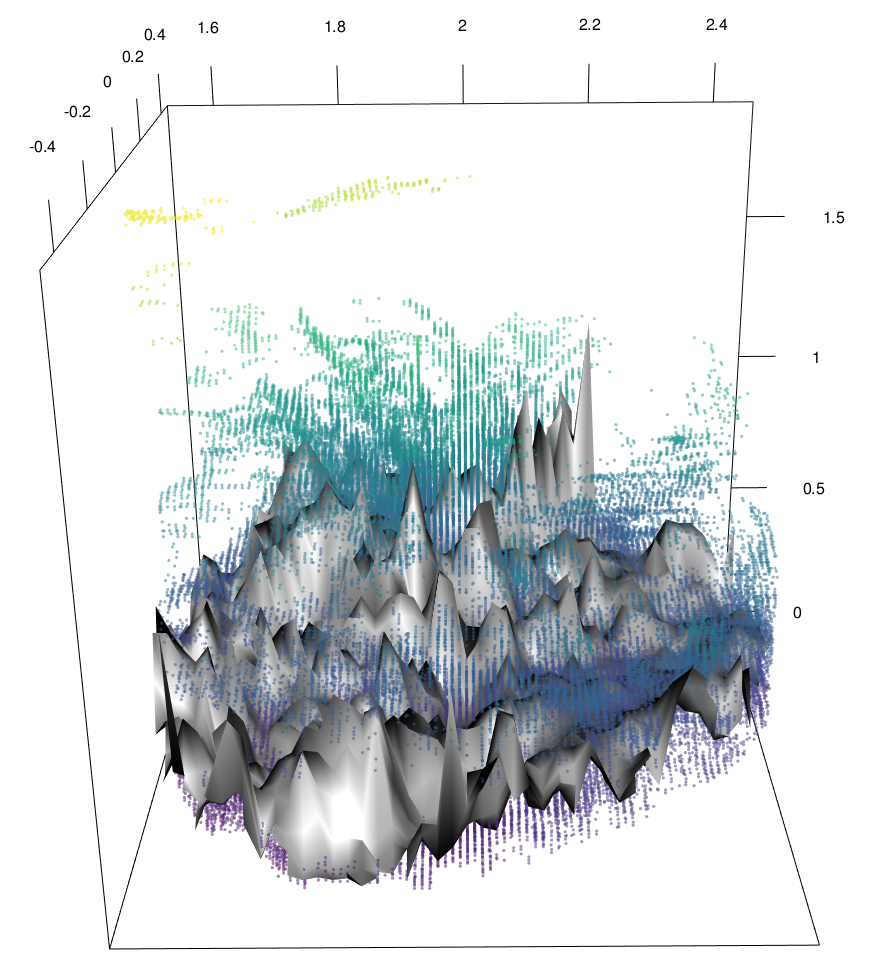
\includegraphics[width=\textwidth]{grass_3d}
	\caption{Point cloud with mean heights for each 2 cm\textsuperscript{2} column labelled and the estimated grassy volume below.}
	\label{grass_3d}
\end{figure}

\section{Canopy rugosity}

The canopy rugosity of each 1 ha plot was estimated. All scans from each plot were merged to a single point cloud, and noise reduction was performed as described above and the cloud was voxelised to 10 cm\textsuperscript{3} cubic voxels. The point cloud was cropped to the plot boundaries, which were located with dGPS similar to the LiDAR targets. 

A canopy height model was produced to describe the upper canopy surface. The 99th percentile of height in each 10 cm\textsuperscript{2} vertical column was extracted. The maximum height was not used as this occasionally constituted a severe outlier which skewed further 
canopy height model smoothing. We used the pit-filling algorithm described in \citet{Khosravipour2014} to smooth the canopy height profile by removing gaps within trees caused by incomplete penetration of the LiDAR beam.

From the canopy height profile we extracted a number of statistics for use in statistical modelling. We calculated the mean and coefficient of variation of canopy height across the plot (canopy rugosity), following \citep{Parker2004}. We calculated the Topographic Ruggedness Index (TRI) as the mean of absolute differences between the heights of each column and the height of its eight surrounding cells \citep{Wilson2007}. From this we estimated the plot level mean TRI and coefficient of variation. 

We also calculated a second measure of canopy rugosity ($R_{c}$) following \citet{Hardiman2011}, using all point cloud data rather than just the top surface:

\begin{equation}
	R_{c} = \sigma{}(\sigma{}G_{z})_{x}
\end{equation}

Where $G_{z}$ is the vertical height axis $z$, $x$ is the horizontal axis, and $\sigma{}$ is the standard deviation.

\section{Data analysis}

All linear mixed effects models werre conducted using the \texttt{\{lmer\}} package in R version 4.0.2 \citep{R2021}.

\subsection{Foliage density profiles}

We conducted a number of linear mixed effects models to assess the effects of tree diversity and stand structure on various aspects of canopy structure. Linear mixed effects models were used to account for the nested sampling structure of subplots within plots, and plots within sites.

For each subplot canopy structure measure, we created a linear mixed effects model with fixed effects for subplot species richness, stem density, and spatial mingling indices.

\subsection{Canopy gap fraction}

We conducted a linear mixed effects model to assess the fit between gap fraction estimates from hemispherical photos and the hemispherical photo simulation produced from the TLS data. We included random slope terms for each 1 ha nested within site. We also assessed the fit of LAI (Leaf Area index) measurements in the same way.

\subsection{Grassy biomass}

To estimate the correlation between grassy volume estimated by TLS and grass biomass estimated from the allometry of DPM height and grassy biomass samples, we conducted a linear mixed effects model of grass biomass vs. grassy volume, with nested random slope terms for each 1 ha plot nested within site. 

We conducted a linear mixed effects model to assess the effects of canopy structure on grassy volume, with random slope terms for each 1 ha plot nested within site. We began with a maximal model which included subplot tree species richness, stem density, TLS gap fraction, layer diversity, height of maximum foliage density, standard deviation of the foliage density profile, and our simple measure of foliage density uniformity. We re-fitted the model with all possible combinations of fixed and random effects and compared AIC, BIC, and log-likelihood to determine which combination of explanatory variables best accounted for variation in grassy volume. Once this `best model' had been identified we extracted effect sizes for each fixed effect as standardized slopes. We also compared random effects for each fixed effect to understand how the two sites differed.

\subsection{Canopy rugosity}

To understand the effect of species composition and stand structure on whole-plot canopy rugosity, we conducted a linear mixed effects model with fixed effects for the shannon diversity index of tree species diversity, stem density, and the coefficient of variation of stem diameter, with random intercept terms for each site.

We extracted slopes for each fixed effect to compare their effect sizes and compared our model with a null model which consisted only of the random effect of site and the fixed effect of stem density.

\printbibliography

\end{document}

